\part En la figura \ref{fig:triang_sem02}, el triángulo {\color{cielogris}FGH} es semejante al triángulo {\color{strawberry}DEF}. ¿Cuál es el valor de $p$?

\begin{minipage}[t]{0.5\linewidth}
    \begin{figure}[H]
        \raggedright
        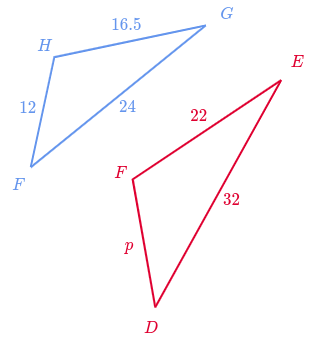
\includegraphics[width =0.9\linewidth ]{Images/triang_sem02}
        \caption{}
        \label{fig:triang_sem02}
    \end{figure}
\end{minipage}%
\begin{minipage}[t]{0.5\linewidth}
    \begin{solutionbox}{7cm}
        Los triángulos semejantes tienen lados proporcionales.

        $\Rightarrow$ podemos establecer proporciones equivalentes y resolver para $p$.

        $\therefore$
        \[
            \dfrac{k}{12} =\dfrac{32}{24} \]    y  \[k =16\]
    \end{solutionbox}
\end{minipage}